\documentclass[12pt,a4paper]{report}
\usepackage{url}
\usepackage{hyperref}
\usepackage{pdfpages}
\usepackage{titlesec, blindtext, color}
\usepackage{amsmath}
\usepackage{amsfonts}
\usepackage{graphicx}
\usepackage{relsize} 
\usepackage{wrapfig}
\usepackage{setspace}
\usepackage{amsthm}
% Allow including SVGs, converting them with Inkscape
\usepackage{svg}
% probably not needed with xelatex engine
%\usepackage[utf8]{inputenc}
% Allows setting fixed width in tables columns
\usepackage{array}
% Allows breaking tables in multiple pages
\usepackage{longtable}
% Syntax highlighted code blocks using Pygment
\usepackage{minted}
% Use custom fonts, used to redefine the monospaced font
\usepackage{fontspec}
% Colors
\usepackage{xcolor}
% Bibliography in ToC
\usepackage[nottoc,notlot,notlof]{tocbibind}
% Typesetting quotes
\usepackage{csquotes}
% Force figure placement
\usepackage{float}
% Boh, lo usa luca
\usepackage{multirow}


% Translate autoref names
\renewcommand{\sectionautorefname}{sezione}
\renewcommand{\tableautorefname}{tabella}
\renewcommand{\figureautorefname}{figura}

% Translate captions
\renewcommand\listingscaption{Listato}
\renewcommand{\figurename}{Figura}
\renewcommand{\bibname}{Riferimenti}
\renewcommand\tablename{Tabella}
\newenvironment{code}{\captionsetup{type=listing}}{}
\renewcommand{\contentsname}{Indice}

% Caption appeareance
\usepackage[font=footnotesize, labelfont=bf]{caption}
\captionsetup[table]{position=below}
\captionsetup[figure]{position=below}

% Set monospaced typeface
\setmonofont{Iosevka}[Scale=0.85]

% Linked ToC
\hypersetup {
    linktoc=all, % both sections and subsections linked
}

% Chapter titles
\graphicspath{ {images/} }
\definecolor{gray90}{gray}{0.90}
\titleformat{\chapter}[hang]{\Huge\bfseries}{\thechapter\hsp\textcolor{gray90}{|}\hsp}{0pt}{\Huge\bfseries}
\newcommand{\hsp}{\hspace{10pt}}

% Confusion matrix preset
\newcommand\MyBox[2]{
  \fbox{\lower0.75cm
    \vbox to 1.7cm{\vfil
      \hbox to 1.7cm{\hfil\parbox{1.4cm}{#1\\#2}\hfil}
      \vfil}%
  }%
}

\begin{document}

\title{%
  \Huge Progetto Basket Shots\\
  \large Predizione dell'esito di tiri nella pallacanestro competitiva utilizzando Support Vector Machines\\
    }
\author{
  Coppola Matteo\\
  \texttt{793329}
  \and
  Palazzi Luca\\
  \texttt{793556}
   \and
  Vivace Antonio\\
  \texttt{793509}
}
\date{Data Technology e Machine Learning, \\ Febbraio 2019}
\maketitle

\tableofcontents

\chapter{Introduzione}
\section{Dominio di riferimento e obbiettivi}
Il settore sportivo professionistico è in costante ricerca di strumenti, modelli e modalità che permettano di analizzare gli andamenti delle partite e le performance dei singoli giocatori.

Il basket americano, ad esempio, utilizza in maniera intensiva indici statistici per monitorare le prestazioni degli atleti durante il corso della stagione. Ne esistono a centinaia e vengono costantemente consultati da allenatori, giornalisti ed osservatori in quanto, talvolta, si rivelano indicatori del valore reale di un giocatore e descrittori di vari aspetti delle partite.
\par
L’NBA, lega professionistica della regione statunitense, oltre ad essere il più grande spettacolo sportivo al mondo è anche un investimento economico di notevole portata e con ampi margini di profitto. Nel 2017 il valore medio di una squadra ha raggiunto 1,1 miliardi di dollari e, per mantenere una continua crescita ed ambire al primo posto in classifica, ogni team cerca di impossessarsi sia dei migliori \textit{players} sul mercato sia degli strumenti più all’avanguardia.
\par
È in quest’ultimo ambito che il Machine Learning può fornire il suo contributo: analizzando le varie performance e gli esiti delle partite passate si possono fare previsioni di vario genere su molti aspetti di questo sport. 
Questo è possibile perchè alcuni servizi e siti, ufficiali e non, mettono a disposizione le statistiche e i dati di cui abbiamo parlato prima in grandi datasets, che noi utilizzeremo come training sets.
\par
Strumenti di previsione e di classificazione possono essere utili anche per chi scommette sugli esiti delle partite, ambito anch’esso estremamente remunerativo e popolare negli Stati Uniti.
\par
Il nostro progetto si pone quindi l'obiettivo di individuare ed utilizzare un metodo di Machine Learning per predire il risultato (\textit{made} o \textit{missed}) di un tiro a canestro in NBA, utilizzando alcuni di tali indici ritenuti più rilevanti e significativi abbinati alle informazioni inerenti alle partite.
\par
Tutto il lavoro prodotto, i dataset iniziali, intermedi e finali, gli script R e Python, le routine Talend e questo documento \LaTeX{} sono disponibili pubblicamente nel repository Git basket-shots \cite{repo}.

\chapter{Data Technology}
\section{Acquisizione}

Dopo aver scelto il dominio applicativo di riferimento e aver deciso gli obiettivi principali, abbiamo scelto due dataset ospitati dalla piattaforma Kaggle.

\subsection{Shot logs}


\texttt{Shot\_logs.csv}\cite{shot_logs} contiene 128 000 record riguardanti i tiri a canestro effettuati da 281 giocatori NBA diversi nella stagione 2014-2015. La fonte originale di questi dati è l’API pubblica del sito dell’NBA.
\begin{center}
	\begin{longtable}[m]{|m{8em} m{7em} m{16em}|} 

		\caption{Campi presi in considerazione del dataset \texttt{shot\_logs.csv}.\label{long}}\\

		\hline
		\bfseries{Attributo} & \bfseries{Tipo di dato} & \bfseries{Descrizione} \\
		\hline
		Location & factor(home, away) & In casa o fuori casa \\
		\hline
		W & factor(win, loss) & Partita vinta o persa dalla squadra del giocatore che ha fatto il tiro \\ 
		\hline
		Final margin & int & Scarto tra punteggi delle due squadre a fine partita \\ 
		\hline
		Shot number & int & Numero del tiro da inizio partita \\ 
		\hline
		Periodo & factor(1,2,3,4) & Periodo della partita, 4 nel basket \\ 
		\hline
		Game clock & Date/Time & Tempo della partita in cui si è effettuato il tiro \\ 
		\hline
		Shot Clock & Date/Time & Secondo in cui il tiro viene rilasciato dall’attaccante. L’intervallo va da 0 a 24, in quanto 24 è il tempo massimo a disposizione della squadra per effettuare un’azione \\ 
		\hline
		Dribbles & int & Numero di dribbling effettuati dall’attaccante prima del tiro \\ 
		\hline
		Touch Time & float & Tempo dal possesso palla in cui ha tirato il giocatore \\ 
		\hline
		Shot Dist & float & Distanza dal canestro al momento del tiro \\ 
		\hline
		PTS Type & factor(2,3) & Tipo di tiro effettuato (da 2 o da 3) \\ 
		\hline
		Shot Result & factor(made, missed) & L’obiettivo che vogliamo predire, esito del tiro (a segno o fallito) \\ 
		\hline
		Closest Defender & String & Nome del difensore più vicino all’attaccante \\ 
		\hline
		Close Def Dist & int & Distanza tra il difensore più vicino e l’attaccante \\ 
		\hline
		Player name & String & Nome dell’attaccante \\ 
		\hline
	\end{longtable}
\end{center}

\texttt{percentage\_previous\_game} è una nuova feature che abbiamo computato dai dati esistenti. Rappresenta la percentuale di successo al tiro fino a quel momento in stagione. Il suo valore è stato ottenuto il seguente script Python che, facendo uso della libreria \textit{Pandas}, aggrega i dati delle partite precedenti a quella a cui si riferisce il tiro in questione.

\begin{code}
\captionof{listing}{datasets/shot\_logs\_nv.py}
\inputminted[breaklines]{python}{../datasets/shot_logs_nv.py}
\end{code}

Nel caso in cui la partita sia la prima della stagione, \texttt{percentage\_previous\_game} assume il valore \texttt{TS}, ovvero la percentuale di successo al tiro riferito a tutta la stagione (\textit{True Shooting}), proveniente dall’altro dataset che abbiamo preso in considerazione, \textit{Seasons stats}.

\subsection{Seasons stats}

\texttt{Seasons\_stats.csv} \cite{season_stats} contiene le statistiche inerenti agli atleti e alle loro performance, dal 1950 al 2017. I dati sono originari del sito Basketball Reference\cite{basketball-reference}, prelevati usando tecniche di \textit{web scraping}.

\begin{center}
	\begin{longtable}[m]{|m{5em} m{7em} m{16em}|} 

		\caption{Campi presi in considerazione del dataset \texttt{Season\_stats.csv}.\label{long}}\\
		\hline
		\bfseries{Attributo} & \bfseries{Tipo di dato} & \bfseries{Descrizione} \\
		\hline

		Year & int & Anno di gioco\\ 
		\hline
		Player & String & Nome del giocatore\\ 
		\hline
		Pos & String & Ruolo nella squadra\\ 
		\hline
		Age & int & Età durante quella stagione\\ 
		\hline
		Games & int & Partite giocate in quella stagione\\ 
		\hline
		MP & int & Minuti totali giocati\\ 
		\hline
		PER & float & \textit{Player Efficiency Rating}\\ 
		\hline
		TS\% & float & \textit{True Shooting Percentage}\\ 
		\hline
		BLK\% & float & \textit{Block Percentage}, la percentuale di blocchi effettuati \\ 
		\hline

	\end{longtable}
\end{center}
\textit{PER} è indicatore tecnico per valutare la bravura di un giocatore. Definito nel 1989 da John Hollinger
\begin{displayquote}
 The PER sums up all a player's positive accomplishments, subtracts the negative accomplishments, and returns a per-minute rating of a player's performance. 
 \end{displayquote}
Il calcolo del suo valore è piuttosto complesso \cite{BRper}.
\par
\textit{TS\%}, misuratore tecnico per valutare l’efficienza di tiro di un giocatore, è invece definito in \cite{BRglossary} come:

$$TS\% = \frac{PTS}{ 2(FGA + (0.44 \times FTA))}\times100$$

Dove \\
PTS = points scored,\\
FGA = field goal attempts,\\
FTA = free throw attempts. \\

% TODO forse questo va in Data Integration?

È stata effettuata un’integrazione, descritta nella \autoref{integrazione},  affinchè ogni tiro registrato in \textit{Shot logs} avesse anche le statistiche e gli indicatori tecnici dell’attaccante (colui che effettua il tiro) e del difensore (colui che attua il blocco per ostacolare il tiro). Dopodichè abbiamo scelto di rendere anonime le istanze del nuovo dataset rimuovendo nomi di attaccanti e difensori, cosicchè gli algoritmi di Machine Learning considerino e prevedano i risultati indipendentemente dai giocatori coinvolti, basandosi sulle loro statistiche, sul contesto di gioco e sugli altri valori forniti.

\subsection{Ipotesi fatte a priori}

Come per ogni altro processo statistico abbiamo innanzitutto dovuto individuare alcune ipotesi ritenute valide, assumendole tali, per poter orientare la parte di Machine Learning verso l’obbiettivo prefissato.
\par
Come fondamentale assunzione, riteniamo che l’esito del tiro a canestro possa essere dedotto in maniera abbastanza regolare dagli  attributi messi a disposizione dai due dataset utilizzati. In realtà, per ogni tentato canestro giocano un’innumerevole serie di fattori fisici ed ambientali: per esempio, l’esito viene anche influenzato da come il giocatore poggia il peso poco prima di tirare.
\par
Lavorando su performance dei giocatori dell’NBA, supponiamo anche che le loro abilità e la loro coerenza di tiro rimangano più o meno costanti (ad eccezione di poche partite sopra o sotto il loro standard, situazioni di \textit{outlier}).
\par
Ricordiamo inoltre che stiamo considerando la minoranza più forte in assoluto nel vasto mondo del basket, top 1\% dei giocatori agonistici. 
\par
%TODO controllare valore?
\par
Quindi, i risultati e le considerazioni che otterremo con il modello costruito, non saranno rilevanti per contesti diversi da quello considerato.
\par
I due dataset forniscono valori a noi utili che risalgono alla stagione di campionato 2014-2015. Volendo utilizzare i risultati per prevedere gli esiti dei tiri NBA della corrente stagione (2018-2019) dobbiamo supporre che non siano stati introdotti grandi cambiamenti nelle strategie e nel modo di allenare i giocatori, affinchè le dinamiche di gioco rimangano ancora molto simili.
\par
Inoltre, risulterà infattibile prevedere l’esito di tiri effettuati da nuovi giocatori entrati nella lega, poichè alcune delle metriche che utilizziamo sono relative allo storico delle loro performance. 
Una possibile soluzione a questo problema è ricavare valori approssimativi per questi indici consultando altre basi di dati che contengono dati relativi alle performance del giocatore in altre leghe.

\subsection{Misure di qualità dei dataset}

% 2 dimensioni di qualità dei dataset singoli
\subsubsection{Season stats}

Vengono definiti 53 attributi per ogni giocatore. Alcuni di questi tuttavia rappresentano delle criticità che sporcano il dataset, abbassandone la qualità sia a livello di schema sia a livello di istanze.
\par
Innanzitutto riscontriamo una mancata correttezza rispetto al modello: gli attributi \texttt{blanl} e \texttt{blank2} sono indubbiamente campi inutili: nessuna istanza ha valori definiti per queste due colonne. Sono probabilmente refusi della fase di scraping dei dati e vanno eliminati perchè non esistenti nel modello ER e perchè intaccano la minimality del dataset.
\par
Molte ennuple hanno valori mancanti soprattutto in alcuni attributi specifici, mostrando un chiaro caso di incompletezza: sul totale di 1283984 valori 154921 sono vuoti, per un’incompletezza che si attesta sullo 0,12\%.

\begin{center}
	\begin{longtable}[m]{|m{3em} m{3em} m{3em} m{3em} m{3em} m{3em} m{3em}|} 

		\caption{Incompletezza di \texttt{Season\_Stats.csv}.\label{long}}\\
		\hline
		\bfseries{Year} & \bfseries{Player} & \bfseries{Pos} & \bfseries{Age} & \bfseries{PER} & \bfseries{TS\%} & \bfseries{BLK\%} \\ 
		\hline
		0,003 & 0,003 & 0,003 & 0,003 & 0,024 & 0,006 & 0,158 \\
		\hline
	\end{longtable}
\end{center}

Infine la chiave principale per le istanze è un ID incrementale che va da 0 a 24692. Si tratta di una chiave non molto utile per il tipo di dataset: le performance dei giocatori andrebbero indicizzati con un ID univoco che si riferisce al singolo atleta. In questo modo sarebbe stato più facile eseguire l’integrazione tra i due dataset e, se avessimo voluto fare un’integrazione più ampia tra dataset di leghe diverse, sarebbe stato più facile rintracciare le statistiche dello stesso giocatore in campionati diversi.

\subsubsection{Shot logs}

Questo dataset presenta meno criticità, risultando più completo. Nonostante ciò, l’attributo \texttt{shot\_clock} presenta un’incompletezza dello 4,35\%: per 5577 istanze su 128069 il suo valore non è specificato.
Infine i valori delle colonne \texttt{player\_name} e \texttt{closest\_def} mancano di correttezza: giocatori con lo stesso id (quindi corrispondenti allo stesso giocatore) sono rappresentati con formati e capitalizzazioni diverse: \texttt{player\_name} infatti il segue il formato \texttt{Cognome, Nome} con le iniziali maiuscole, mentre in \texttt{closest\_def} il formato è \texttt{nome cognome} tutto in minuscolo. È un caso di eterogeneità a livello di istanze.

\par
Questo problema caratterizza il 100\% delle istanze.

\section{Preparazione}
\label{preparazione}
Abbiamo fatto notare che nel file \texttt{shot\_logs.csv} i nomi degli attaccanti (attributo \texttt{player\_name}) e i nomi dei difensori (attributo \texttt{closest\_defender}) hanno un formato diverso. Per eseguire una corretta integrazione con l’altro dataset è necessario quindi uniformare preliminarmente questi valori, permettendone l’identificazione, sia esso l’attaccante o il difensore nel tiro in questione. 
\par
Non si tratta di \textit{deduplication} perchè quest’ultima mira ad individuare istanze che si riferiscono ad uno stesso concetto all’interno dello stesso database, mentre qui non abbiamo istanze duplicate, ma valori diversi che in domini differenti si riferiscono alla stessa entità.
\par
Inizialmente avevamo optato per una funzione che separasse i nomi in \textit{token}, li ordinasse lessicograficamente e che li risolvesse rilevando un match per una totale distanza di edit minore di 3 o maggiore solo in caso di diminutivi (per esempio: \texttt{J.J. Barea} e \texttt{Barea Jose Juan}).

Questa funzione è stata implementata in Python, nel file \texttt{datasets/match.py} \cite{repo}.
\par
Il metodo funzionava correttamente, ma ci siamo poi accorti che due attributi del dataset (\texttt{player\_id} e \texttt{closest\_def\_id}) corrispondevano univocamente. Abbiamo quindi utilizzato la componente \textit{tMap} in Talend per uniformare i nomi di attaccanti e difensori: abbiamo ricercato giocatori con lo stesso id e abbiamo sostituito il loro nome nella colonna \texttt{player\_name} (nome dell’attaccante) con quello della colonna \texttt{closest\_defender}.
\par
Il risultato di tale operazione ci ha permesso una più agevole integrazione con l’altro dataset, poichè quest’ultimo non possiede un ID univoco per i giocatori e il processo integrativo deve essere necessariamente effettuato facendo corrispondere i nomi degli atleti.
\par
%TODO
Infine bisogna specificare che per ovviare all’assenza di 5577 occorrenze nel campo \texttt{shot\_clock}, abbiamo deciso di considerare il valore medio per giocatore.
\par
Per i nostri scopi, dal dataset \textit{Seasons Stats} otteniamo un sottoinsieme delle statistiche dei giocatori riferite all’anno 2015. Al suo interno è possibile trovare fino a quattro duplicati della coppia di attributi Year e Player, in quanto nella lega è permesso giocare in quattro differenti squadre ogni stagione. Ciò è stato risolto aggregando i valori degli attributi sopra citati, gestendo le statistiche numeriche (\texttt{BLK}, \texttt{TS}, \texttt{PER}) considerando la media stagionale e considerando invece l’occorrenza più recente per gli attributi \texttt{Pos} ed \texttt{Age}.
\par
Alcuni record che riguardavano giocatori di cui non abbiamo informazioni per la stagione interessata, sono stati rimossi. E.g. \textit{Atila Dos Santos} compare in alcune istanze del primo dataset ma lo stesso non è presente nel secondo dataset che descrive le caratteristiche dei giocatori.

\section{Integrazione}
\label{integrazione}

L'analisi esplorativa dei due datasets, anche in vista dell'applicazione dei metodi di Machine Learning, ha prodotto come risultato due nuovi datasets composti da un insieme ridotto di attributi, ritenuti rilevanti e non ridondanti per lo studio e gli obiettivi prefissati. Il numero di record è rimasto inalterato.
\par
L'integrazione dei due nuovi datasets ha avuto luogo in due passi separati. Inizialmente, sono stati utilizzati con una componente \textit{tMap} per associare al dataset dei tiri le statistiche degli attaccanti. Dopodiché, questo dataset consistente dei nuovi attributi è stato utilizzato assieme al dataset delle statistiche per associare, con un'altra componente \textit{tMap}, le informazioni relative al difensore.
\par
\begin{figure}[H]
\caption{Pipeline d'integrazione dati implementata con \textit{Talend Studio}}
	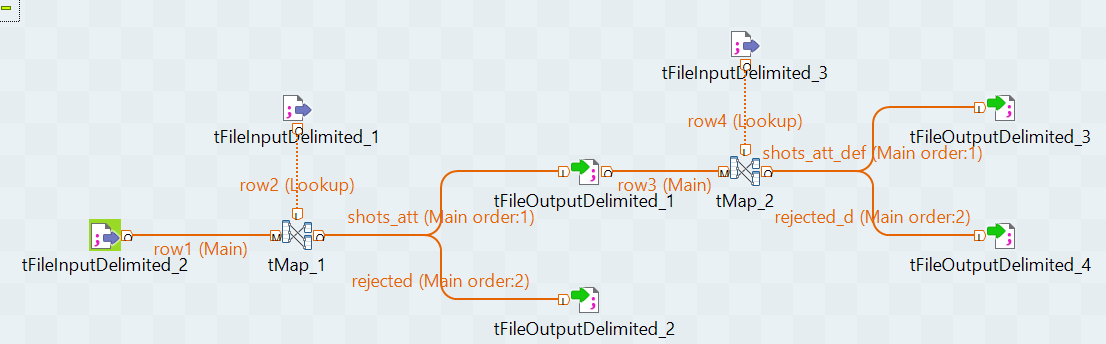
\includegraphics[width=\linewidth]{pipeline_talend1.png}
\end{figure}

Non utilizzando un ID univoco che identifica un giocatore per effettuare l'integrazione tra i due datasets ma i nomi stessi degli atleti, abbiamo optato per l'utilizzo della stessa funzione descritta nella \autoref{preparazione}, così da uniformare i nomi presenti (scritti in minuscolo ordinati lessicograficamente) nei due datasets. 
\par

Effettuata l'integrazione, per verificare la consistenza del matching in ciascuno dei due passi è stato creato un file denominato \textit{rejected} in cui sono state inserite le istanze respinte, non trovando una corrispondenza perfetta.
\par
Circa una decina di nomi sono risultati in questa lista: sono risolti manualmente nella routine \texttt{EditShotLogs\_0.1.java}, eseguita in pipeline da Talend, poichè sarebbe stato problematico e dispendioso usare funzioni di edit distance appositamente parametrizzate per così pochi e particolari casi.

\begin{code}
\captionof{listing}{Metodo matchNames da EditShotLogs\_0.1.java}
\begin{minted}{java}
public static String matchNames(String name1) {
	String[] def = {"Barea, Jose Juan", "Hardaway Jr., Tim", 
		"Aminu, Al-Farouq", "Nene", "Mbah a Moute, Luc",
		"Hayes, Charles", "Lucas III, John", "Taylor, Jeff",
		"Rice Jr., Glen", "Datome, Gigi", "McAdoo, James Michael"};
	String[] stats = {"J.J. Barea", "Tim Hardaway", 
		"Al-Farouq Aminu", "Nene Hilario", "Luc Mbah",
		"Chuck Hayes", "John Lucas", "Jeffery Taylor",
		"Glen Rice", "Luigi Datome", "James Michael"};
	String[] results = {"barea jj", "hardaway tim", 
		"al-farouq aminu", "nene hilario", "luc mbah",
		"chuck hayes", "john lucas", "jeffery taylor",
		"glen rice", "datome luigi", "james mcadoo michael"};
	if (Arrays.asList(def).contains(name1) || 
		Arrays.asList(stats).contains(name1)) {
		for (int i = 0; i < def.length; i++) {
			if (name1.equals(def[i]) || 
				name1.equals(stats[i])) {
				return results[i];
			}
		}  
	}
	String[] names1 = name1.replaceAll("[^a-zA-Z ]", "")
		.toLowerCase().split("\\s+");
	Arrays.sort(names1);
	String nuova = "";
	for (int i = 0; i < names1.length; i++) {
		nuova += names1[i];
		nuova += " ";
	}
	nuova = nuova.trim();
	return nuova;
}
\end{minted}
\end{code}

\subsection{Misure di qualità del dataset integrato}

\subsubsection{Currency, Volatility e Timeliness}
Un aspetto importante dei dati coinvolti nel nostro processo di integrazione è il loro cambiamento nel tempo. I database a nostra disposizione contemplano l'anno di campionato 2014-2015 ma è ovvio che questi vengano continuamente aggiornati e integrati con il corso dei campionati.

\textit{Currency}, definita come la velocità degli aggiornamenti \cite{batini2006}, è calcolabile con la seguente formula\cite{doi:10.1287/mnsc.44.4.462}
\begin{equation}
Currency = Age + (DeliveryTime - InputTime)
\end{equation}
\textit{Age} misura l'età dei dati quando vengono ricevuti, \textit{DeliveryTime} è l'istante in cui il prodotto che utilizza queste informazioni è consegnato all'utente finale mentre \textit{InputTime} è l'istante in cui il dato è stato effettivamente ottenuto.
Il termine $(DeliveryTime - InputTime)$ misura quindi il periodo di tempo che trascore prima che il prodotto che utilizza i nostri dati sia pronto ed effettivamente utilizzabile.

Poichè l'anno corrente è 2019, i dati hanno una \textit{Age} di 4 anni. $(DeliveryTime - InputTime)$ risulta quindi trascurabile e \textit{Currency} è equivalente  ad \textit{Age}.

Supponendo inoltre che le statistiche dell'NBA rimangano rilevanti per le 3 stagioni successive, la \textit{volatilità} dei dati è uguale a 3 anni.

\textit{Timeliness}, calcolata con 

\begin{equation}
\max\{{0, 1 - \frac{Currency}{Volatility}}\}
\end{equation}

Vale quindi 0, rappresentando una cattiva tempestività del nostro dataset.

\subsubsection{Completability}
Essendo i nostri dataset originari di servizi Web e riflettendo eventi reali distribuiti durante l'anno, ne vengono costantemente pubblicate versioni aggiornate.

La \textit{Completabilità} è un'interessante metrica che ci permette di visualizzare la dinamica di evoluzione temporale della completezza.

Consideriamo una funzione $C(t)$, definita come il valore della completezza all'istante t, con $t \in [t_{pub}, t_{max}]$, dove $t_{pub}$ è l'istante iniziale di pubblicazione dei dati e $t_{max}$ il tempo massimo in cui verrà completato l'ultimo degli aggiornamenti dei dati previsiti.

La \textit{completabilità} dei dati è quindi definibile come \cite{batini2006}:

\begin{equation}
\int_{t_{curr}}^{t_{max}} C(t)
\end{equation}

Con $t_{curr}$ l'instante in cui essa viene calcolata ($t_{curr} < t_{max}$).

La \autoref{completabilitypic_gen} generalizza come si presenta, dove $c_{i}$ valore di completezza stimato per un generico $t_{i}$.

% TODO: definizione di A

La Completabilità è definita dall'area segnata come \textit{Cb}. Il confronto con $A$ permette di definire gli intervalli $[Alto, Media, Bassa]$ per la completabilità.


\begin{figure}
\caption{Rappresentazione grafica della completabilità \cite{batini2006}}
\label{completabilitypic_gen}
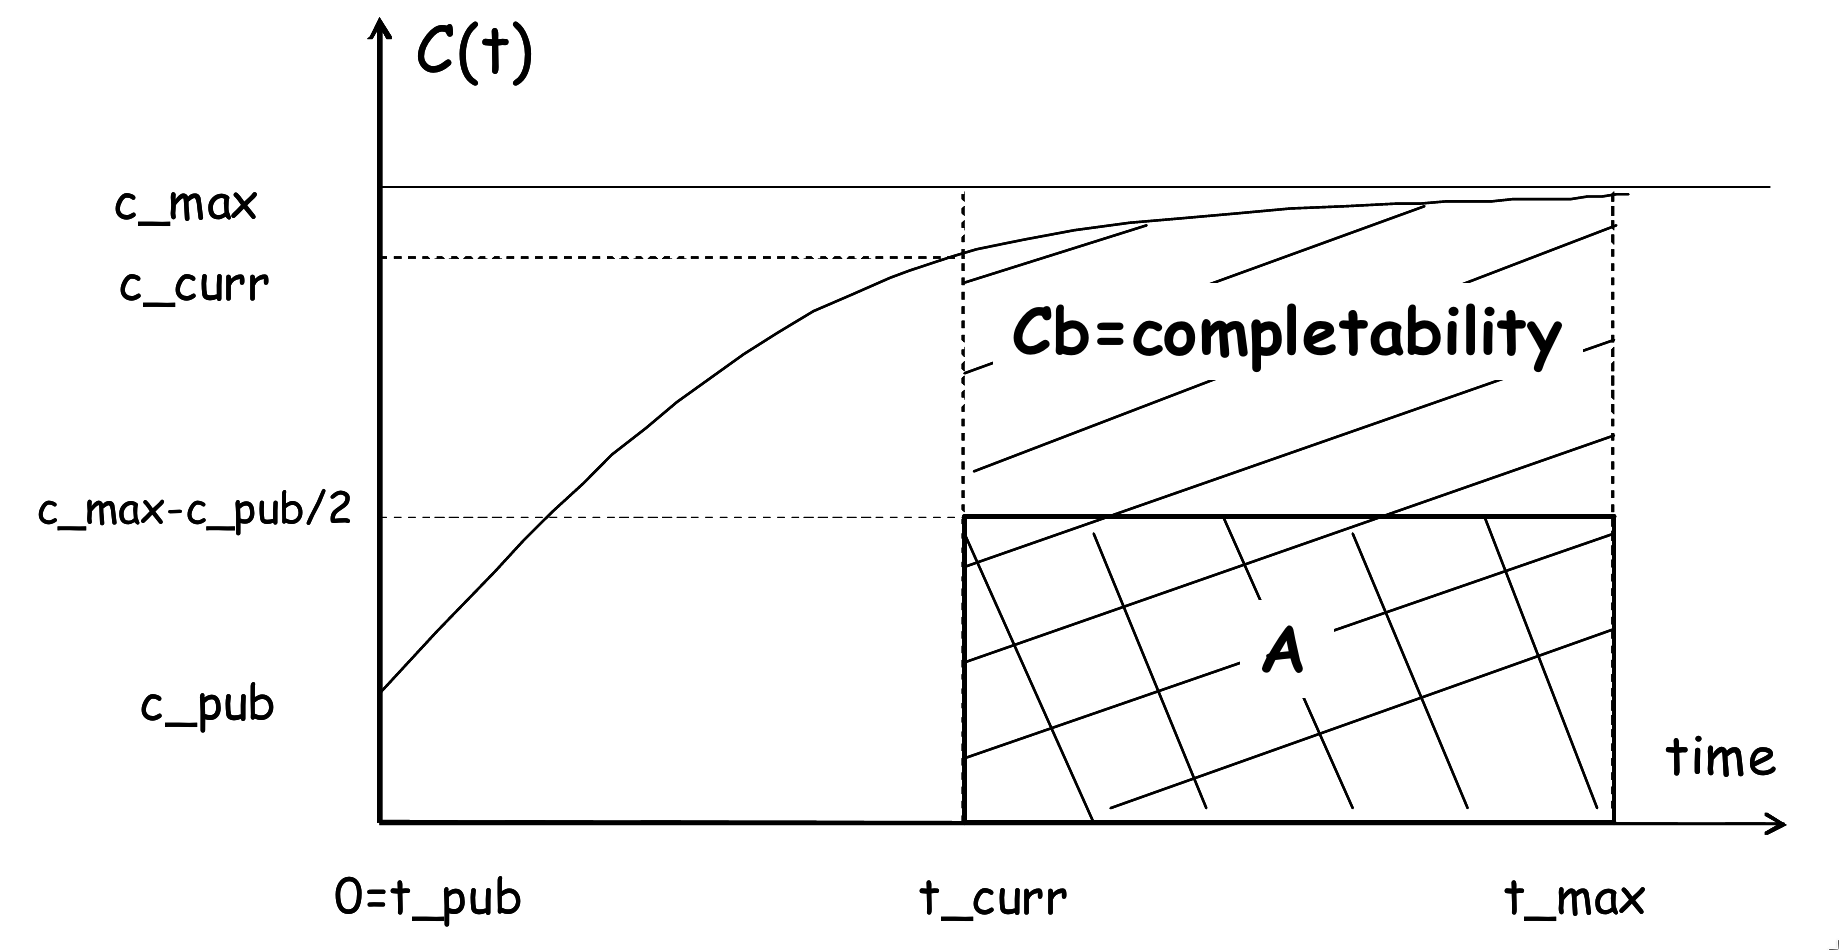
\includegraphics[width=\linewidth]{completability_gen.png}
\end{figure}

\par

Per dare un'idea di che completabilità esibiscono i dataset che consideriamo supponiamo che:


\begin{itemize}
	\item Il ritardo con cui otteniamo i dati sulle partite appena avvenute sia trascurabile, i.e. ad un istante $t$ si abbiano i dati delle partite fino a $t-1$;
\end{itemize}
	% TODO: DECIDERE SE USARE %
	Stimiamo la completezza percentuale dei dati, in un istante \textit{t}, con 
	\begin{equation}
	C(t) = \frac{\sum\limits_{y=c-p-1}^{c-1} M_{y} + m_{c,t}}{\sum\limits_{y=c-p-1}^{c} M_{y}} \times 100
	\end{equation}
	Dove \begin{itemize}
		\item $M_y$ è il numero totale di partite nella stagione $y$;
		\item $m_{c,t}$ il numero totale di partite nella stagione $y$ fino all'istante $t$;
		\item $c$ la stagione considerata
		\item $p$ numero di stagioni precedenti a quella che si vuole considerare che si suppongono rilevanti e parte del dataset.
	\end{itemize}

Considerando tutti gli istanti $t$ in cui siano giocate delle partite, ottenute da \cite{nba_schedule} e utilizzando $y = 2019, c = 3$ (considerando quindi i dati delle stagioni 2019, 2018, 2017, 2016, con 2019 stagione oggetto del dataset), la completabilità evolve secondo la \autoref{completabilitypic} attestandosi su un valore medio.

Scegliendo una finestra temporale più estesa la completabilità mostra un andamento periodico.

Infatti da inizio stagione (Ottobre) fino alla sua fine (Maggio) continuano ad essere forniti dati nuovi dopo ogni singola partita; nel periodo da Maggio a Ottobre invece non ci sono partite e nessun nuovo dato viene generato; infine ad Ottobre inizia un nuovo campionato, rendendo obsoleti i dati più vecchi della finestra mentre si abbassa la completezza.


% TODO: Aggiungere C(t) sull'asse Y, sostituire Date con Time nell'asse X.
\begin{figure}
\caption{Rappresentazione grafica della completabilità nel nostro esempio}
\label{completabilitypic}
\includegraphics[width=\linewidth]{completability}
\end{figure}
\section{Analisi descrittiva del dataset integrato}

Dato il tipo di informazione che desideriamo ottenere dal dataset integrato, abbiamo valutato una serie di statistiche che caratterizzano fortemente i dati, scrivendo un semplice script Python che manipolasse opportunamente il dataset. All'interno dello script, commentati, si trovano le statistiche.

\begin{code}
\captionof{listing}{datasets/shot\_logs\_nv.py}
\inputminted[breaklines]{python}{../dataintegration/count.py}
\end{code}

Inoltre abbiamo rappresentato graficamente la relazione tra numero di giocatori e tiri \texttt{made} mostrata nella \autoref{made_shots_hist} e \texttt{missed} mostrata nella \autoref{missed_shots_hist}:

\begin{figure}
\caption{Frequenza di tiri con esito positivo}
\label{made_shots_hist}
\includegraphics[width=\linewidth]{made_shots_hist}
\end{figure}

\begin{figure}
\caption{Frequenza di tiri con esito negativo}
\label{missed_shots_hist}
\includegraphics[width=\linewidth]{missed_shots_hist}
\end{figure}


\chapter{Machine Learning}
%INTRO
La scelta del modello di machine learning da utilizzare è in gran parte determinata dalle caratteristiche dei dati a disposizione.

Iniziamo dunque con un analisi del nostro dataset per individuare le caratteristiche che descrivono e in che modo i valori che assumono sono distribuiti nelle nostre istanze.

\section{Analisi esplorativa}

\par
Il dataset integrato risultante possiede per ciascuno dei 128 000 tiri informazioni relative al tiro e dati relativi agli atleti coinvolti nello scontro che ha portato allo stesso.
\par

In Shot logs sono stati esclusi alcuni attributi (descritti nella \autoref{tabella_shot_logs}) riguardanti la partita come \texttt{W}, \texttt{Final margin} e \texttt{Matchup}, ritenuti non rilevanti per le sorti di un tiro a canestro.
Anche \texttt{Period} e \texttt{Game clock} sono stati ritenuti superflui, in quanto è già presente l'attributo \texttt{Shot number}, così come non significativo è stato valutato l'attributo \texttt{Pts type} (deducibile dall'attributo \texttt{Shot distance}). 
\par
Analogamente, in Seasons stats sono stati esclusi decine di indici statistici non determinanti, oltre agli attributi (descritti in \autoref{tabella_seasons_stats}) come \texttt{Games} e \texttt{MP}.

\par

Alcuni dati che sarebbe stato interessante avere, ma assenti nelle nostri fonti riguardano fattori più circostanziali al tiro, che sono reperibili grazie al "visual tracking", come ad esempio la parabola del tiro stesso, la velocità dell'attaccante e del difensore, le coordinate sul rettangolo di gioco dei due giocatori e così via. Queste e altre dinamiche di gioco permetterebbero di creare modelli più approfonditi in modo da fornire predizioni più fedeli.

\par
I valori da predire sono distribuiti in modo non uniforme. Il 55\% (70 157 record) sono tiri \textit{missed}, mentre il 45\% (57 900 record) sono tiri \textit{made}(\autoref{dist_shot_result}).

\begin{figure}
\caption{Distribuzione degli esiti nel dataset integrato}
\label{dist_shot_result}
	\includegraphics[width=\linewidth]{shot_result}
\end{figure}

\par

\begin{figure}
\caption{Importanza delle feature, secondo il modello prodotto}
\label{importance_fig}
\fontsize{9pt}{1em}
	\includegraphics[width=\linewidth]{importance}
\end{figure}

\par

\textit{Importance}, mostrata nella \autoref{importance_fig}, rappresenta il contributo informativo delle feature considerate. Le principali risultano \texttt{shot\_dist}, \texttt{close\_def\_distance} e \texttt{dribbles}.

\begin{figure}
\caption{Correlazione tra gli attributi più rilevanti}
\label{plot_shot_dist_def}
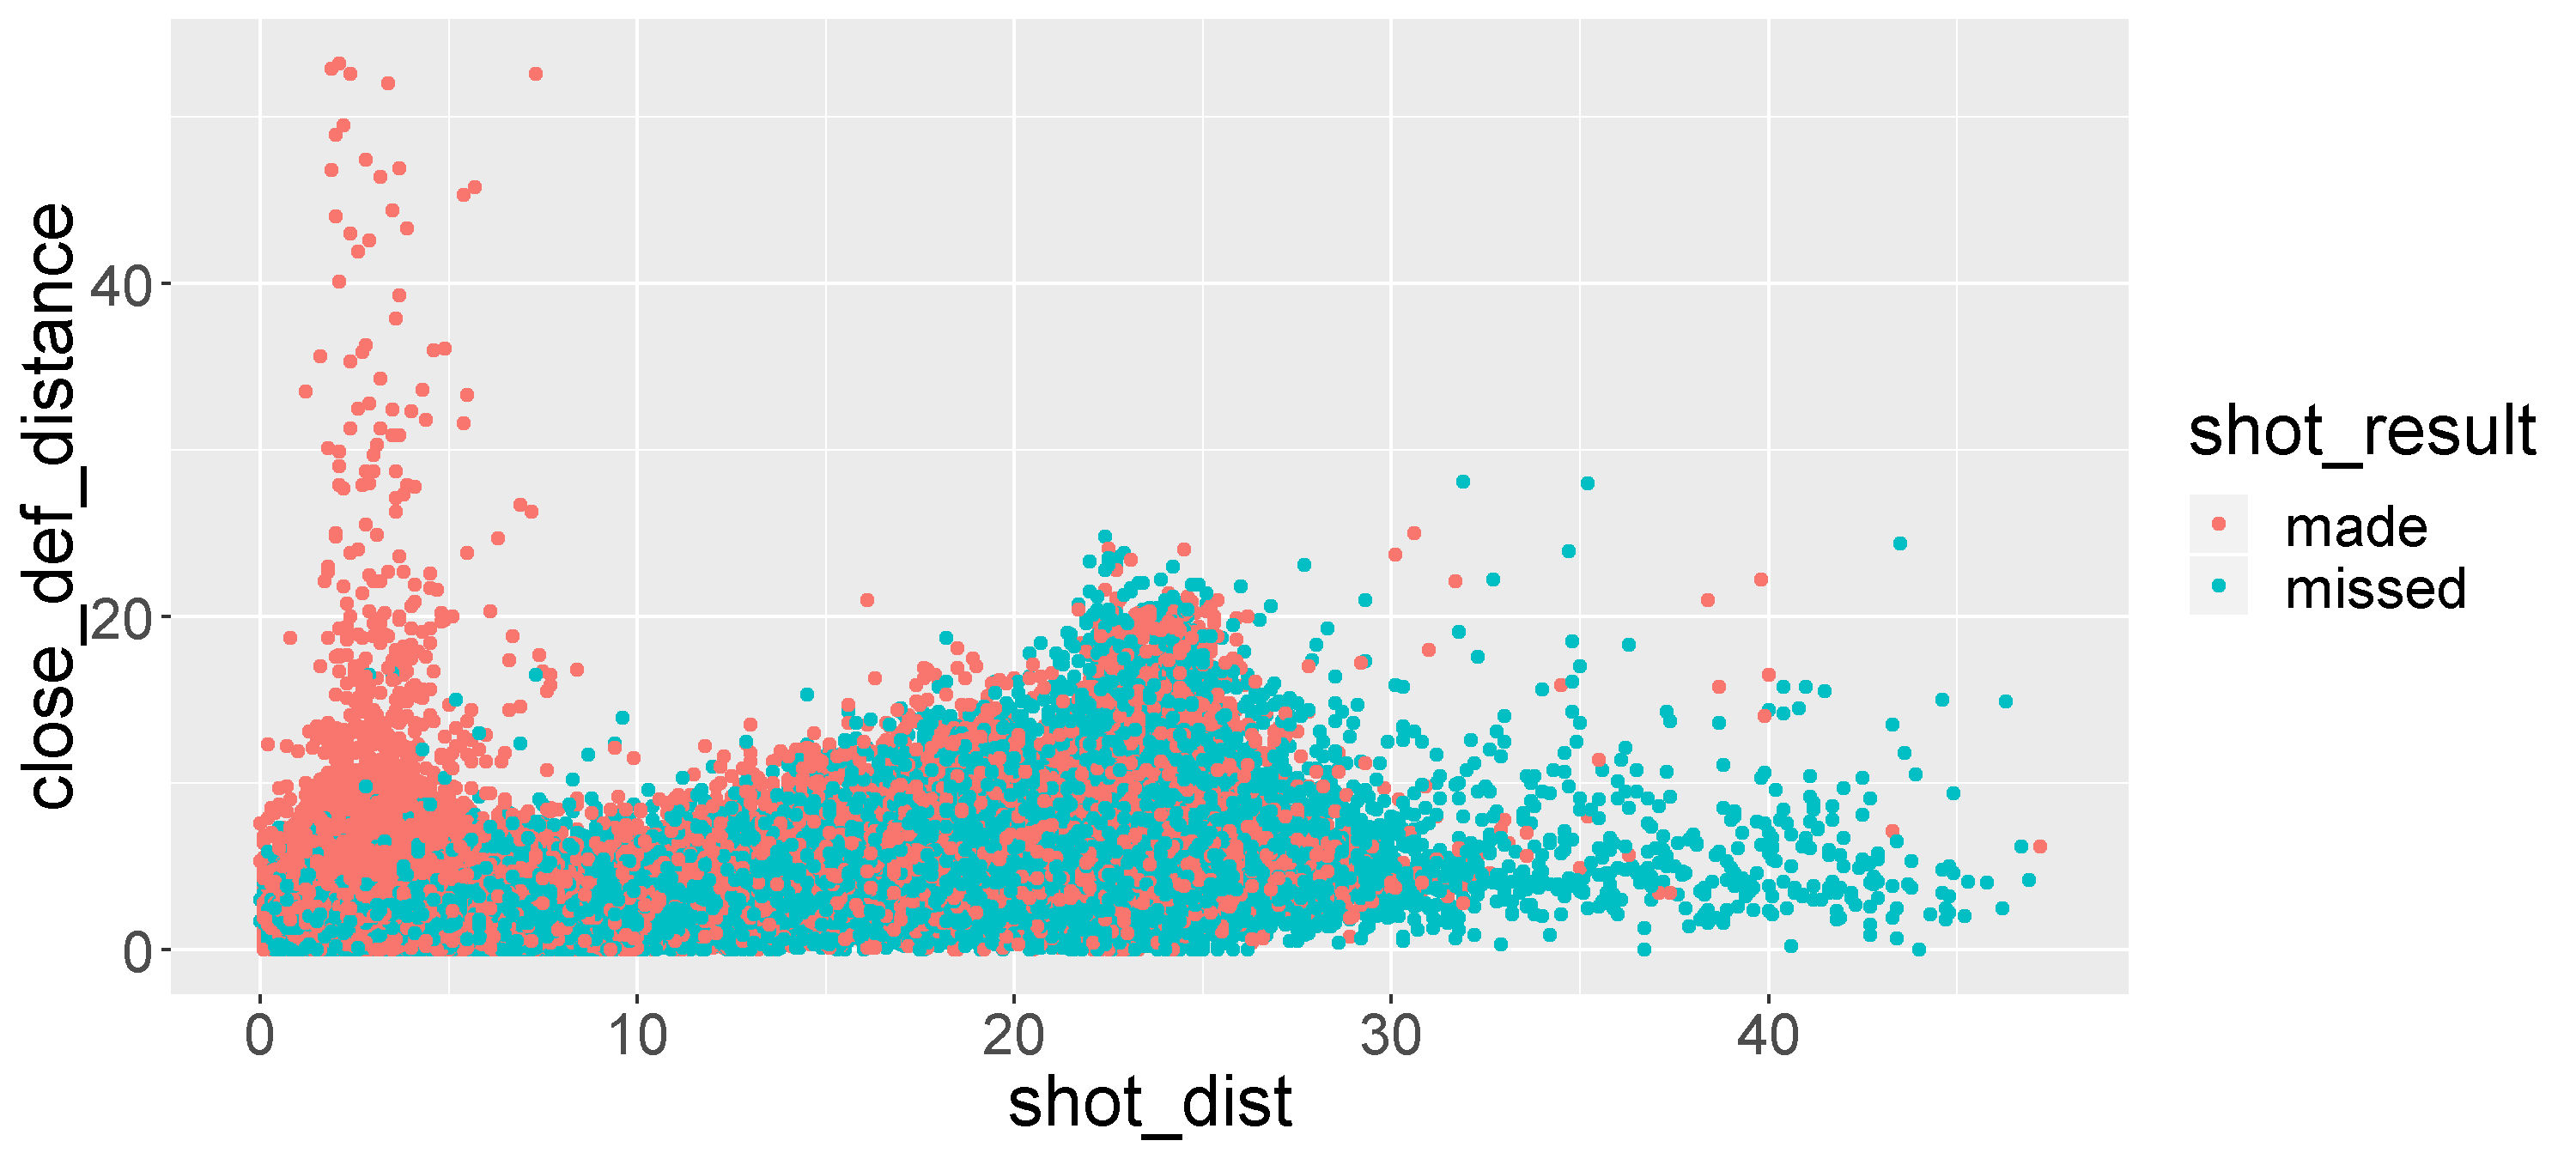
\includegraphics[width=\linewidth]{plot_shot_dist_def.png}
\end{figure}

Il grafico è stato interpretato considerando due regioni: la regione con prevalenza \texttt{made}, ossia quella compresa tra $[0, 10]$ nell'asse delle ascisse e $[5, 60] $ nell'asse delle ordinate, e la regione con prevalenza \texttt{missed}, ossia quella compresa tra $[25, 40]$ nell'asse delle ascisse e $[0, 20] $ nell'asse delle ordinate.
Abbiamo intepretato le distribuzioni di queste due regioni rintracciando quello che succede sul campo: i tiri effettuati dal pitturato (area sottostante al canestro), seppur con il difensore molto vicino, hanno una probabilità di essere messi a segno molto alta. I tiri effettuati dalla distanza, invece, sono notoriamente più difficili ed in questo caso è la probabilità di fallimento ad essere più elevata.

\par

\begin{figure}
\caption{Distanza media del tiro rispetto al ruolo del giocatore}
\label{position_shot_dist}
\includegraphics[width=\linewidth]{shot_dist_with_position}
\end{figure}

Il grafico in \autoref{position_shot_dist} mostra che C, il componente della squadra che domina il pitturato, tira in media da una distanza inferiore ai 10 piedi, seguito da PF. I giocatori in questo ruolo prendono quindi tiri ad indice di difficoltà più basso rispetto alla media.
Non abbiamo a disposizione informazioni relative a peso e altezza, ma i dati \cite{basketball-reference} mostrano che in media in questi due ruoli giocano gli atleti più fisicamente dotati: soffrendo meno il contatto con l'avversario riescono a raggiungere più facilmente il canestro.

Al contrario, gli altri tre ruoli (PG, SF e SF) tirano da una distanza che si aggira intorno ai 15 piedi. Solitamente sono meno prestanti dal punto di vista fisico ma con un'abilità al tiro superiore, che li porta a prendere anche tiri di notevole difficoltà dalla distanza.

\begin{figure}
\caption{Successo dei tiri rispetto al ruolo del giocatore}
\label{position_shots}
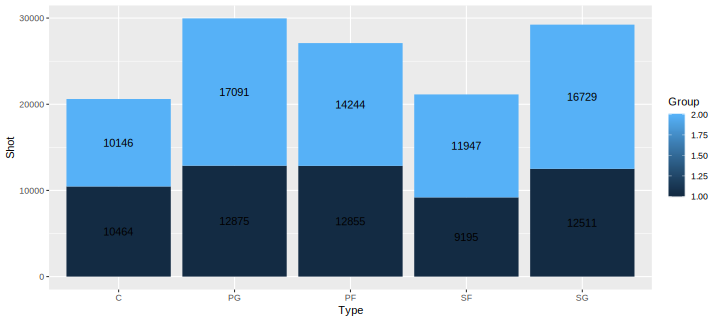
\includegraphics[width=\linewidth]{made_missed_barplot}
\end{figure}

La \autoref{position_shots} conferma questa intepretazione: PF ha una percentuale di missed pari a 0.53, mentre addirittura inferiore (0.49) è la la percentuale di missed per C, per di più l'unico ruolo ad avere un numero di tiri made maggiori rispetto ai missed ma anche quello con il minor numero di tiri effettuati.
Gli altri tre ruoli (PG, SF, SG) hanno una percentuale di missed pari a 0.57.

\section{Scelta del modello}
% Scelta di C (complexity paramater) e Sigma (gaussian kernel parameter)

Il nostro dataset integrato ha un buon numero di attributi, sia numerici che categorici.
Abbiamo quindi deciso di utilizzare SVM, un algoritmo di apprendimento automatico supervisionato ampiamente utilizzato per problemi di classificazione. Il suo punto di forza è l'utilizzo del cosiddetto \textit{kernel trick}, strumento matematico per mappare l'input in uno spazio multi-dimensionale. SVM performa bene con dataset composti da tanti attributi e numerose osservazioni, adeguato sotto questo punto di vista al nostro caso.
La presenza di attributi categorici porterebbe a preferire gli alberi di decisione, ma esistono alcune tecniche che possono trasformare queste tipologie di campi affinchè siano compatibili anche con le SVM.
\section{Preparazione del dataset}

La fase di Data integration è stata impostata in modo tale da produrre un dataset pulito e direttaemnte sottoponibile ad un modello di Machine Learning.

Ricordiamo che gli attributi relativi ai nomi degli atleti, resi necessari dalla mancanza di un ID univoco, vengono rimossi dopo aver effettuato l'integrazione.

Il primo passo effettivo, quindi, è stato il preprocessing dei dati. I valori nulli di ciascun attributo erano stati rimossi durante l’integrazione. È da verificare, invece, la presenza di valori inconsistenti nel dominio dell’attributo preso in considerazione.
Per \texttt{touch\_time} sono stati trovati valori non positivi. Considerando che questo attributo rappresenta periodi di tempo non nulli e minori di 24 secondi, valori non negativi non sono ammessi e sono stati rimossi.
Non sono stati trovati altri attributi con valori anomali.

\par

È stata stata applicata una normalizzazione del dataset per gli attributi numerici. È un procedimento che viene applicato frequentemente perché gli attributi sono calcolati con unità di misura differenti. In questo modo si evita che un attributo abbia un peso maggiore di un altro. È stato utilizzato per ciascun attributo il metodo
\begin{equation}
\text{(min max)}\quad x = \dfrac{x - min(x)}{max(x) - min(x)}
\end{equation}
molto utilizzato in letteratura in alternativa a
\begin{equation}
\text{(z score)}\quad x = \dfrac{x - \mu}{\sigma}
\end{equation}
 in quanto gli attributi sono limitati in un range. Con \textit{min max} i valori di ciascun attributo vengono posti tra 0 e 1.

\par
Non essendo SVM una tecnica che gestisce attributi categorici, è stata applicata una tecnica di \textit{one-hot encoding} per gestirli. In questo modo vengono creati tanti nuovi attributi quante sono le categorie di ciascun attributo. Il nuovo attributo è 1 se l’attributo originale aveva quel determinato valore, 0 altrimenti.
\section{Implementazione del modello}

Nonostante gli aspetti positivi, è difficile determinare se la SVM sia la tecnica ideale per allenare il nostro dataset. Non esiste infatti un motivo davvero discriminante che porti a preferirla rispetto ad altri modelli come le reti neurali oppure gli alberi di decisione.
Inizialmente abbiamo provato ad implementare la SVM con il package R chiamato e1071, ma il dataset utilizzato contiene un numero eccessivo di istanze e la computazione risultava troppo onerosa (cannot allocate vector in R of size xx Gb). Abbiamo sperimentato anche con il package liquidSVM ma non erano presenti di default funzionalità utili allo sviluppo del progetto come la ROC e l'AUC, quindi abbiamo optato per il package rminer che implementa l’algoritmo della SVM di Kernlabs, basato sul paper di Platt (LINKARE PAPER) in cui viene descritto il metodo ad oggi più efficiente per ottenere stime probabilistiche sulla classificazione del test set con una SVM.

\subsubsection{Creazione del training set}


Una volta importato e suddiviso il dataset per l’apprendimento automatico, la seguente riga produce e allena il modello:

\texttt{}

Sebbene il nostro sia un problema di classificazione, settare il parametro task a \textit{prob} ci permette di ottenere dalla logica di SVM il valore $ f(z) $ calcolato per ogni istanza di test $z$, piuttosto che il semplice segno aritmetico $sign(f(z))$ che indica una posizione minore o maggiore rispetto alla threshold, determinando la classe di appartenenza:

% f(z)=wTϕ(z)+b,=∑i∈SVαiyiκ(xi,z)+b 

%(https://stats.stackexchange.com/questions/134156/can-i-use-svm-classification-probability-for-ranking)


Con task uguale ”prob” il valore $f(z)$ viene automaticamente scalato in un range $[0, 1]$ con la tecnica chiamata \textit{Platt scaling}, producendo quindi una stima della probabilità di classificazione.
Aggiungendo alla funzione fit il seguente parametro \texttt{search="heuristic10"}

consentiamo la ricerca semiautomatica degli iperparametri ottimali su 10 range diversi per massimizzare la predizione del modello.

Dopo una ricerca euristica su un sample di 25000 istanze, le metriche più accurate sono state ottenute con il valore C della SVM uguale 1 e kernel “RBFDOT” ossia Radial Basis Function Kernel.
La funzione di discriminazione di tale Kernel è:
Formula di 

%https://it.wikipedia.org/wiki/Funzione_radiale_di_base


\pagebreak
\section{Esperimenti e analisi dei risultati}

Il comando \textit{mmetric} ci permette di ottenere metriche e stime di performance sul nostro modello:
\begin{minted}{r}
metrics=mmetric(testset$shot_result,prediction,metric=c("ALL"))
\end{minted}

%TODO: aggiungere valori
\begin{table}[H]
\centering
  \begin{tabular}{l l} 
  Accuracy complessiva & xx\\
  Precision per la classe \textit{made} & xx\\
  Precision per la classe \textit{missed} & xx\\
  Recall per la classe \textit{made} & xx\\
  Recall per la classe \textit{missed} & xx\\
  F-measure per la classe \textit{made} & xx\\
  F-measure per la classe \textit{missed} & xx\\
  Area Under Curve complessiva & xx\\
    \end{tabular}
    \caption{Metriche del modello SVM}
\end{table}

\begin{table}[H]

%TODO: aggiungere valori
\centering
\noindent
\renewcommand\arraystretch{1.5}
\setlength\tabcolsep{0pt}
\begin{tabular}{c >{\bfseries}r @{\hspace{0.7em}}c @{\hspace{0.4em}}c @{\hspace{0.7em}}l}
\centering
  \multirow{10}{*}{\rotatebox{90}{\parbox{1.1cm}{\bfseries\centering Actual value}}} & 
    & \multicolumn{2}{c}{\bfseries Prediction outcome} & \\
  & & \bfseries p & \bfseries n & \bfseries total \\
  & p$'$ & \MyBox{True}{Positive} & \MyBox{False}{Negative} & P$'$ \\[2.4em]
  & n$'$ & \MyBox{False}{Positive} & \MyBox{True}{Negative} & N$'$ \\
  & total & P & N &
\end{tabular}
 \caption{Confusion Matrix di SVM}
 \label{confusion_matrix_svm}
\end{table}

L'esecuzione della Cross Validation non migliora molto questi risultati:

%TODO: aggiungere valori
\begin{table}[H]
\centering
  \begin{tabular}{l l} 
  Accuracy complessiva & 61.16\\
  Precision per la classe \textit{made} & 61.32\\
  Precision per la classe \textit{missed} & 61.09\\
  Recall per la classe \textit{made} & 38.49\\
  Recall per la classe \textit{missed} & 79.90\\
  F-measure per la classe \textit{made} & 47.29\\
  F-measure per la classe \textit{missed} & 69.24\\
  Area Under Curve complessiva & 0.62\\
    \end{tabular}
    \caption{Metriche risultate dell'esecuzione della cross validation su SVM}
\end{table}

\begin{table}[H]

%TODO: aggiungere valori
\centering
\noindent
\renewcommand\arraystretch{1.5}
\setlength\tabcolsep{0pt}
\begin{tabular}{c >{\bfseries}r @{\hspace{0.7em}}c @{\hspace{0.4em}}c @{\hspace{0.7em}}l}
\centering
  \multirow{10}{*}{\rotatebox{90}{\parbox{1.1cm}{\bfseries\centering Actual value}}} & 
    & \multicolumn{2}{c}{\bfseries Prediction outcome} & \\
  & & \bfseries p & \bfseries n & \bfseries total \\
  & p$'$ & \MyBox{4 357} & \MyBox{6 962} & P$'$ \\[2.4em]
  & n$'$ & \MyBox{2 749} & \MyBox{10 932} & N$'$ \\
  & total & P & N &
\end{tabular}
 \caption{Confusion Matrix di SVM dopo la cross validation}
 \label{confusion_matrix_svm_cv}
\end{table}

\begin{figure}[H]
  % QUA CI VA ROC PRIMA DI CV
  \centering
  \begin{subfigure}{.5\textwidth}
  \centering
  \caption{Prima}
  \label{roc-svm-missed-25k}
  \includegraphics[width=.8\linewidth]{roc-svm-missed-25k}
\end{subfigure}%
\begin{subfigure}{.5\textwidth}
  \centering
  \caption{Dopo}
  \label{roc-svm-made-25k}
  \includegraphics[width=.8\linewidth]{roc-svm-made-25k}
\end{subfigure}%
  \caption{ROC su SVM}
\end{figure}


Il risultato, intuitivamente un po' basso, è in realtà in linea con le aspettative: i fattori che influenzano un tiro a canestro sono molteplici, mentre le informazioni in nostro possesso sono limitate. Il fatto che sia comunque  superiore al \textit{random guessing} dimostra che esistono dei fattori nel dataset che tendono effettivamente ad influenzare il successo o il fallimento del tiro.

\par
% to do: verificare correttezza
Considerando la classe \textit{made} quella positiva e la classe \textit{missed} quella negativa, dalle metriche ottenute possiamo fare alcune valutazioni: per entrambe le classi il valore di precision è simile ed è sul 60\%, da cui deduciamo una proporzionalità di falsi positivi e falsi negativi.
Guardando le recall invece notiamo che per la classe \textit{missed} tendono ad esserci pochi falsi negativi, mentre la vera criticità è il numero eccessivo di falsi positivi per \textit{made}. In altre parole, un tiro legittimo tende ad essere considerato un fallimento.

Le F-measure sono valori che permettono di confrontare direttamente le due classi. Precision e recall sono spesso diverse e quindi è complicato determinare quale classe abbia effettivamente meno errori: la F-measure, ottenuta computando la media armonica di queste due metriche, permette di quantificare le performance delle due classi in maniera comparabile. Nel nostro caso era deducibile che la f-measure di \textit{missed} fosse molto più alta di quella di \textit{made}: la disparità nelle recall influisce molto sul calcolo complessivo.

Essendo un problema di apprendimento automatico binario, la Area Under Curve, intesa come AUROC (Area Under Receiver Operating Characteristic), è solo una. Tale metrica corrisponde all'area sottostante la ROC, ottenuta muovendo gradualmente la threshold della SVM e rappresentando sul grafo ogni volta i valori di TPR (\textit{True Positive Rate}) e FPR (\textit{False Positive Rate}).
Più grande (vicino a 1) è il valore della AUROC, più è grande la distinzione tra True Positive e True Negative: nel nostro caso vale 0.64.

\par
Sia eseguendo SVM sull'intero dataset, diviso opportunamente in training set (80\%) e trainset (il restante 20\%), sia eseguendolo con una 10-fold cross validation, il valore di accuracy complessivo tra le due esecuzioni non si discosta troppo. Ciò porta a concludere che il dataset è formato da istanze poco sofferenti di bias e difficilmente rischia di andare in overfitting.

\pagebreak
\subsection{Alberi di Decisione}
Per verificare come si comportassero altri modelli diversi dalla SVM, abbiamo dato in input il nostro dataset e abbiamo allenato un modello utilizzando gli alberi di decisione.
Innanzitutto è stata eseguita un'euristica per individuare il valore migliore di CP, ossia quello con \textit{xerror} minimo. Questo parametro indica di quanto debba migliorare il relative error complessivo per poter eseguire uno split nel nodo dell'albero.
Il risultato però è stato un albero con un solo split:

\begin{figure}[H]
\caption{Alberi di decisioni}
\label{dt_fig}
  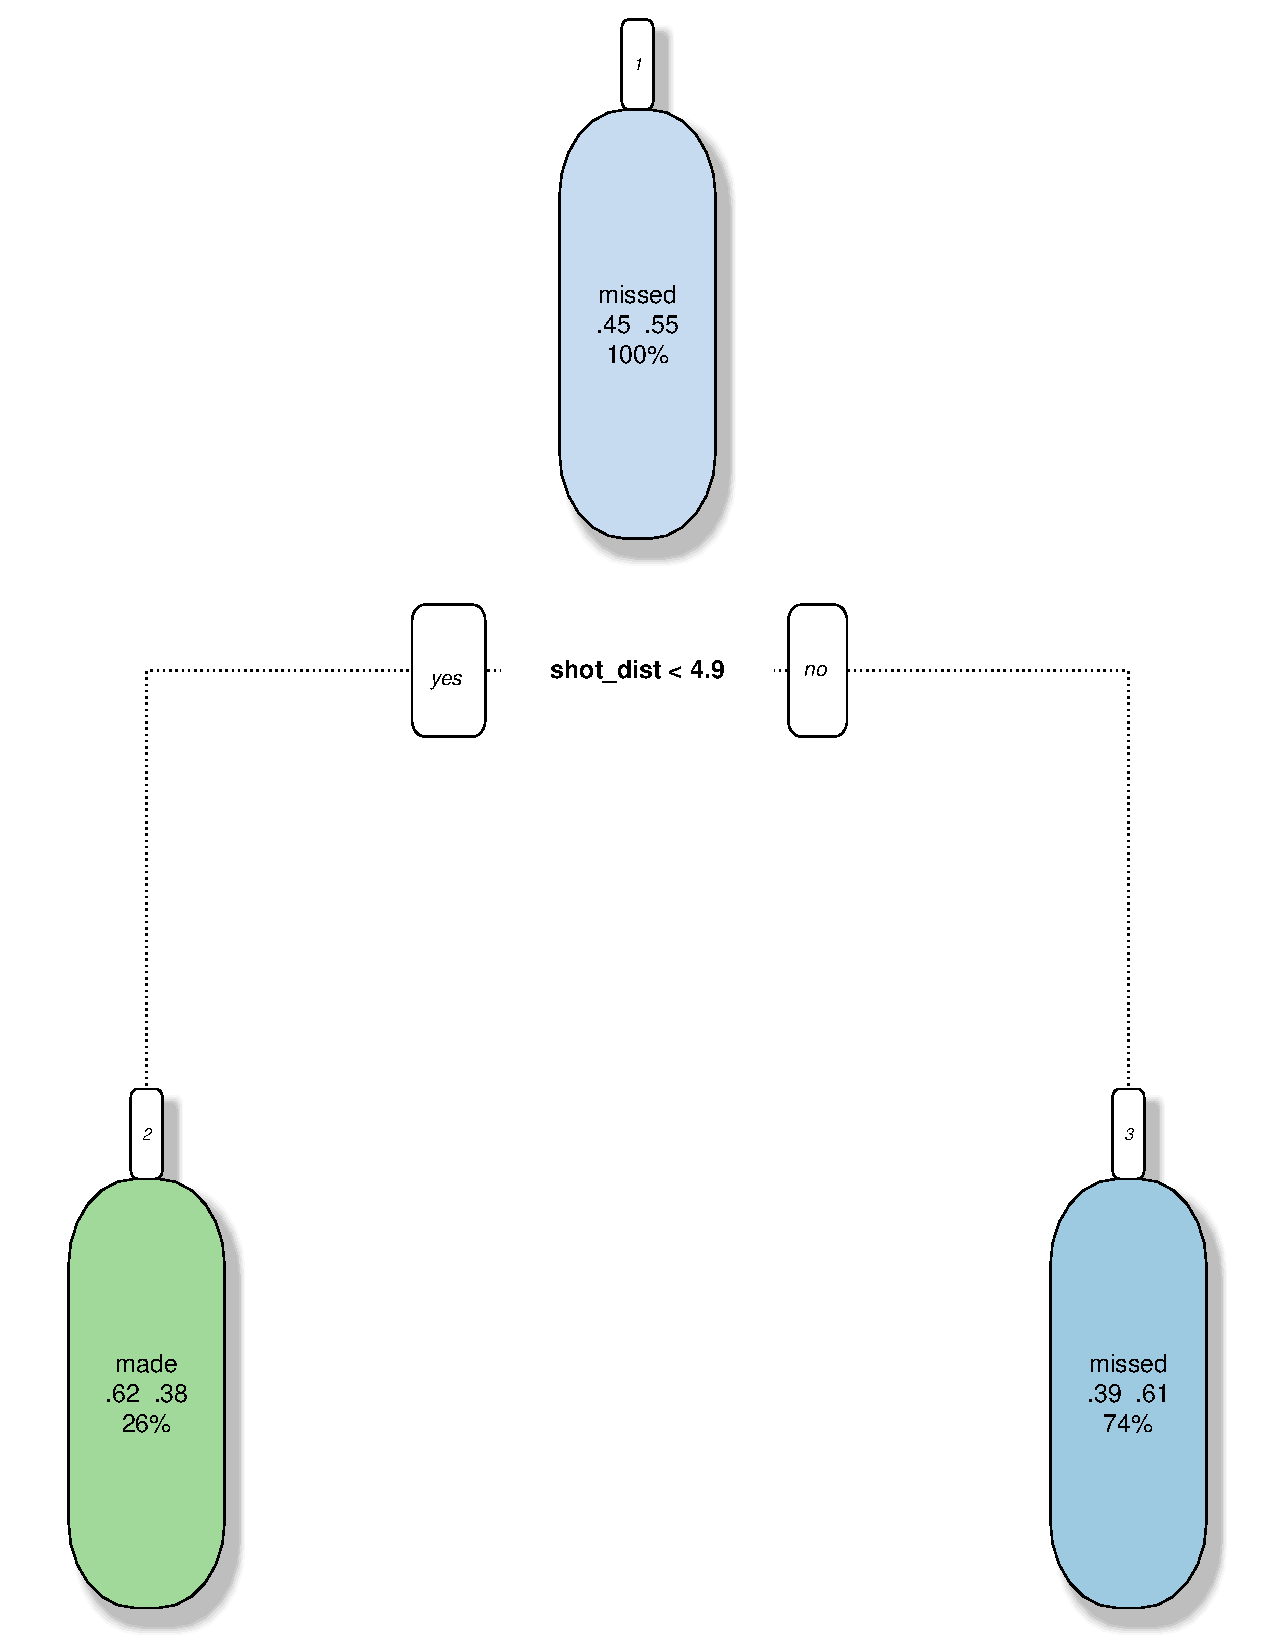
\includegraphics[width=\linewidth]{DECISIONTREE}
\end{figure}


Un'analisi delle metriche e del contributo informativo delle feature considerate ci mostra il perchè di un albero così corto:
\begin{table}[H]
\centering
  \begin{tabular}{l l} 
shot\_dist &77\\
shot\_clock &8\\
touch\_time &8\\
close\_def\_distance &7\\
percentage\_prev\_games &1\\
    \end{tabular}
    \caption{Importance in DT}
\end{table}

\begin{table}[h!]
\centering
  \begin{tabular}{l l} 
  Accuracy complessiva & 61.06\\
  Precision per la classe \textit{made} & 62.12\\
  Precision per la classe \textit{missed} & 60.68\\
  Recall per la classe \textit{made} & 35.71\\
  Recall per la classe \textit{missed} & 82.01\\
  F-measure per la classe \textit{made} & 45.35\\
  F-measure per la classe \textit{missed} & 69.75\\
    \end{tabular}
    \caption{Metriche risultate dell'esecuzione della cross validation su Decision Tree}
\end{table}

L'importance di \textit{shot\_dist} è nettamente più alta di qualsiasi altro attributo.
Questi valori dimostrano che il decision tree non è adeguato per il nostro problema in quanto non coinvolge attributi che per noi sono influenti e probabilmente generalizzerà male con istanze nuove.
Inoltre questo albero di decisione ottiene delle metriche peggiori della nostra SVM.

\begin{table}[H]

\centering
\noindent
\renewcommand\arraystretch{1.5}
\setlength\tabcolsep{0pt}
\begin{tabular}{c >{\bfseries}r @{\hspace{0.7em}}c @{\hspace{0.4em}}c @{\hspace{0.7em}}l}
\centering
  \multirow{10}{*}{\rotatebox{90}{\parbox{1.1cm}{\bfseries\centering Actual value}}} & 
    & \multicolumn{2}{c}{\bfseries Prediction outcome} & \\
  & & \bfseries p & \bfseries n & \bfseries total \\
  & p$'$ & \MyBox{20 639}{} & \MyBox{37 162}{} & P$'$ \\[2.4em]
  & n$'$ & \MyBox{12 587}{} & \MyBox{57 357}{} & N$'$ \\
  & total & P & N &
\end{tabular}
 \caption{Confusion Matrix di DT}
 \label{confusion_matrix_dt}
\end{table}

\bibliographystyle{unsrt}
\bibliography{bibliography}

\end{document}